\documentclass[11pt,a4paper]{article}
\usepackage[margin=1in]{geometry}
\usepackage{amsmath,amssymb}
\usepackage{graphicx}
\usepackage[hidelinks]{hyperref}

\def\eqdef{\overset{\mathrm{def}}{=}}

\begin{document}

\begin{center}
    \textbf{SGD versus Robust SGD under Gradient Uncertainty}
\end{center}

\section{Derivation and interpretation}

We use $\alpha_k>0$, $\rho\geq 0$, and a symmetric positive definite
matrix $S_k$. The observed mean gradient and its uncertainty set are
\[
    g_k=\frac{1}{b}\sum_{i=1}^{b}v_{k,i},
    \qquad
    \mathcal G_k=\{g_k+S_k^{1/2}u:\|u\|_2\leq\rho\}.
\]
Here $S_k^{1/2}$ is the symmetric positive definite square root of $S_k$.
R-SGD chooses a step $d_k$ and sets $\theta_{k+1}=\theta_k+d_k$.

\subsection*{(a) Inner maximum}

Write $c=\mu+S^{1/2}u$. Since $S^{1/2}$ is symmetric,
\[
    c^\top x=\mu^\top x+u^\top S^{1/2}x.
\]
By the Cauchy--Schwarz inequality,
\[
    \mu^\top x+u^\top S^{1/2}x
    \leq \mu^\top x + \|u\|_2\|S^{1/2}x\|_2
\]
Equality is achieved when $u$ is parallel with $S^{1/2}x$, so the optimal choice is 
\[
    u^*=\rho\frac{S^{1/2}x}{\sqrt{x^\top Sx}}
    \quad \Longrightarrow \quad
    c^*=\mu + \rho\frac{Sx}{\sqrt{x^\top Sx}}
\]
Therefore
\[
    \max_{c=\mu+S^{1/2}u,\ \|u\|_2\leq\rho}c^\top x
    =\mu^\top x + \rho\frac{x^\top Sx}{\sqrt{x^\top Sx}} = \mu^\top x + \rho\sqrt{x^\top Sx}.
\]

In a local gradient model,
$f(\theta_k+d)\approx f(\theta_k)+h^\top d$, where $h$ is an uncertain
gradient. Hence $x$ becomes the step $d$, $\mu$ becomes $g_k$,
and $S$ becomes $S_k$. The term $f(\theta_k)$ is constant with respect
to $d$, so it does not affect the chosen step.

\subsection*{(b) Equivalent problem and uniqueness}
Define
\begin{equation}
Q_k(D) \eqdef g_k^\top d+\rho\sqrt{d^\top S_kd} +\frac{\|d\|_2^2}{2\alpha_k}.
\label{eq:robust}
\end{equation}
Problem 
\[
\max_{h \in \mathcal G_k} \left\{h^\top d +\frac{\|d\|_2^2}{2\alpha_k}\right\}
\]
is equivalent to problem in (a) since second term is constant in $h$, then
\[
\max_{h \in \mathcal G_k} \left\{h^\top d +\frac{\|d\|_2^2}{2\alpha_k}\right\} = Q_k(d) \quad \text{and} \quad d_k=\operatorname*{arg\,min}_{d} Q_k(d)
\]
For $\rho=0$, the optimality condition $\nabla Q_k(d) = 0$ is
\[
    g_k+\alpha_k^{-1}d_k=0 
    \quad \Longrightarrow \quad
    d_k=-\alpha_k g_k.
\]
Consequently, $\theta_{k+1}=\theta_k-\alpha_k g_k$, which is SGD.

The function $\sqrt{d^\top S_kd}=\|S_k^{1/2}d\|_2$ is convex, and linear term is convex. 
The quadratic term is strongly convex because $\alpha_k>0$.
Thus $Q_k$ is strongly convex and has at most one minimizer.
Also,
\[
    Q_k(d)\geq-\|g_k\|_2\|d\|_2
                   +\frac{\|d\|_2^2}{2\alpha_k},
\]
which is convex quadratic function in $\|d\|$.
Therefore, there exists a ball $B = \{d : \| d \| > r\}$ such that $Q_k(d) > M$ for every $d \not \in B$ and $M > 0$. Also $Q(0) = 0 < M$ and $0 \in B$. Using that $Q(k)$ is strongly convex and continuous we get that it has unique minimizer inside $B$.
Therefore the robust step exists and is unique.

\subsection*{(c) When the robust step is zero}

If $g_k^\top S_k^{-1}g_k\leq\rho^2$ then using 
Cauchy--Schwarz inequality gives
\[
    g_k^\top d=(S_k^{-1/2}g_k)^\top(S_k^{1/2}d)
    \geq-\sqrt{g_k^\top S_k^{-1}g_k}\sqrt{d^\top S_kd} \ge - \rho \sqrt{d^\top S_kd}.
\]
then 
\[
    Q_k(d)\geq\frac{\|d\|_2^2}{2\alpha_k}.
\]
Since $Q_k(0)=0$, the unique minimizer is $d_k=0$.

To prove the reverse implication, suppose that $d_k=0$.
Then $Q_k(td)\geq Q_k(0) = 0$ for every $d$ and every $t>0$, so
\[
    0\leq\frac{Q_k(td)}{t}
    =g_k^\top d+\rho\sqrt{d^\top S_kd}
      +\frac{t}{2\alpha_k}\|d\|_2^2.
\]
Letting $t\downarrow 0$ gives
\[
    g_k^\top d+\rho\sqrt{d^\top S_kd}\geq 0
    \qquad\text{for every }d.
\]
Set $z=S_k^{1/2}d$. Since $S_k^{1/2}$ is invertible, $z$ ranges over
all vectors. In particular, the inequality must hold for every unit
vector $z$. Therefore,
\begin{gather*}
    0\leq\min_{\|z\|_2=1}
       \left\{(S_k^{-1/2}g_k)^\top z+\rho\right\}=\rho-\|S_k^{-1/2}g_k\|_2 =\rho-\sqrt{g_k^\top S_k^{-1}g_k}
       \quad \Rightarrow \quad
       g_k^\top S_k^{-1}g_k \le \rho^2
\end{gather*}
Together with the previous implication, this proves
\[
    d_k=0
    \quad\Longleftrightarrow\quad
    g_k^\top S_k^{-1}g_k\leq\rho^2.
\]
A zero step does not imply $\nabla f(\theta_k)=0$.
For example, in one dimension let
\[
    f(\theta)=\tfrac12\theta^2,
    \qquad \theta_k=1,\qquad g_k=1,\qquad S_k=1,\qquad\rho=1.
\]
Then $d_k=0$ since $g_k^\top S_k^{-1}g_k (= 1) \le \rho^2 (= 1)$ but
$f'(\theta_k)=1$.

\subsection*{(d) Nonzero step and the isotropic case}

For $d\neq 0$, the objective in \eqref{eq:robust} is differentiable, with
\[
    \nabla_d\sqrt{d^\top S_kd}
    =\frac{S_kd}{\sqrt{d^\top S_kd}}.
\]
Setting its gradient to zero gives
\begin{equation}
    g_k+\rho\frac{S_kd_k}{\sqrt{d_k^\top S_kd_k}}
        +\alpha_k^{-1}d_k=0.
    \label{eq:optimality}
\end{equation}
Because $Q_k$ is convex, this condition is also sufficient for a
nonzero point to be the minimizer.

If $S_k=sI$ with $s>0$, then \eqref{eq:optimality} becomes
\[
    g_k+\rho\sqrt{s}\frac{d_k}{\|d_k\|_2}
        +\alpha_k^{-1}d_k=0 
        \quad \iff \quad 
        g_k=-\left(\frac{\rho\sqrt{s}}{\|d_k\|_2}+\alpha_k^{-1}\right)d_k
\]
Thus $d_k$ is parallel to $-g_k$. Taking norms gives
\[
    \|g_k\|_2=\rho\sqrt{s}+\frac{\|d_k\|_2}{\alpha_k}
    \quad \iff \quad
    \|d_k\|_2 = \alpha_k\left( \|g_k\|_2 - \rho\sqrt{s} \right)
\]
Part (c) gives that $d = 0 \iff g_k^\top S_k^{-1}g_k \le \rho^2$ which is in our case gives $d = 0 \iff \|g_k\|^2_2 \le \rho^2s$. So solution can be written as
\[
    d = \begin{cases}
		0, & \text{if $\|g_k\|_2 \le \rho\sqrt{s}$}\\
        -\alpha_k\left( \|g_k\|_2 - \rho\sqrt{s} \right)\frac{g_k}{\|g_k\|}, & \text{otherwise}
	\end{cases}
\]
which is equivalent to
\[
d = -\alpha_k\left( 1 - \frac{\rho\sqrt{s}}{\|g_k\|} \right)_{+}g_k
\]
If $g_k=0$, all terms in $Q_k(d)$ are nonnegative and $Q_k(0)=0$,
so $d_k=0$ for every $\rho\geq 0$.

In isotropic case R-SGD step differs from SGD step only in multiplier 
\[
C_{\text{is}} \eqdef \left( 1 - \frac{\rho\sqrt{s}}{\|g_k\|} \right)_{+}
\]
so 
\[
d = \underbrace{-\alpha_k g_k}_\text{SGD step} C_{\text{is}}.
\]
from previous discusion follows that $C_{\text{is}} < 1$, so R-SGD step have the same direction as SGD bad have smaller magnitude. 

In anisotropic case w.l.o.g. assume that we work in orthonormal eigenbasis of $S$, so $S = \operatorname{diag}(\lambda_1, \ldots, \lambda_p)$ where $\forall i \; \lambda_i \ge 0$, and let $r_k=\sqrt{d_k^\top S_kd_k}>0$. Then from \eqref{eq:optimality} follows 

\[
d_k=-\alpha_k
        \left(I+\frac{\alpha_k\rho}{r_k}\operatorname{diag}(\lambda_1, \ldots, \lambda_p)\right)^{-1}g_k
\]
which in coordinate view results in
\[
    (d_k)_j=
    -\frac{\alpha_k(g_k)_j}
           {1+\alpha_k\rho\lambda_j/r_k}.
\]
Each component is reduced relative to SGD, so
$\|d_k\|_2\leq\alpha_k\|g_k\|_2$. Directions with larger
$\lambda_j$ have larger uncertainty and receive a stronger reduction.
Since these reductions can differ, anisotropic uncertainty can change
both the length and the direction of the step.

\subsection*{(e) Decrease of the objective}

Assume $\nabla f(\theta_k)\in\mathcal G_k$ and that $\nabla f$ is
$L$-Lipschitz continuous. By part (a),
\begin{equation}
    \begin{gathered}
    \nabla f(\theta_k)^\top d_k
    \leq\max_{h\in\mathcal G_k}h^\top d_k
    =g_k^\top d_k+\rho\sqrt{d_k^\top S_kd_k} = \\ =
    g_k^\top d_k+\rho\frac{d_k^\top S_kd_k}{\sqrt{d_k^\top S_kd_k}} = \left(g_k^\top +\rho\frac{d_k^\top S_k}{\sqrt{d_k^\top S_k d_k}}\right)d_k.
    \end{gathered}
    \label{eq:containment}
\end{equation}
By \eqref{eq:optimality}
\[
g_k^\top +\rho\frac{d_k^\top S_k}{\sqrt{d_k^\top S_k d_k}} = -\alpha_k^{-1} d_k
\]
Using it in \eqref{eq:containment} implies
\[
\nabla f(\theta_k)^\top d_k \le -\alpha_k^{-1} \|d_k\|^2_2
\]

The Lipschitz assumption gives the smoothness bound. Indeed, for any $d$,
\begin{align*}
    f(\theta_k+d)-f(\theta_k)-\nabla f(\theta_k)^\top d
    &=\int_0^1
      [\nabla f(\theta_k+td)-\nabla f(\theta_k)]^\top d\,dt\\
    &\leq\int_0^1 Lt\|d\|_2^2\,dt
     =\frac L2\|d\|_2^2.
\end{align*}
Using $d=d_k$ and the bound on the directional derivative gives
\[
    f(\theta_k+d_k)
    \leq f(\theta_k)
        -\left(\alpha_k^{-1}-\frac L2\right)\|d_k\|_2^2.
\]
Thus the proposed inequality holds.

For $L>0$, a sufficient condition for strict decrease when $d_k\neq 0$
is $0<\alpha_k<2/L$.
If $f$ is linear and so $L=0$, any $\alpha_k>0$ gives strict decrease for a nonzero step.

Gradient containment is needed in \eqref{eq:containment}: the worst
gradient in the uncertainty set must bound the true directional
derivative. A set built from a finite batch need not contain the true
gradient. Without containment, the objective can increase even when
$\alpha_k<2/L$. For example, consider two training targets, $2$ and $-2$,
with squared losses
\[
    \ell_1(\theta)=\frac{(\theta-2)^2}{2},
    \qquad
    \ell_2(\theta)=\frac{(\theta+2)^2}{2}.
\]
The mean training loss is
\[
    f(\theta)=\frac{\ell_1(\theta)+\ell_2(\theta)}{2}
    =\frac{\theta^2}{2}+2,
    \qquad L=1.
\]
At $\theta_k=1$, the true gradient is $f'(1)=1$.
If we choose first example to estimate the gradient,
then $g_k=\ell_1'(1)=1-2=-1$.
With $S_k=1$, $\rho=1/2$, and $\alpha_k=1$, the set
$\mathcal G_k=[-3/2,-1/2]$ does not contain the true gradient.
By the formula in part (d), the robust step is
\[
    d_k=-\left(1-\frac12\right)(-1)=\frac12,
    \qquad \theta_{k+1}=1+\frac12=\frac32.
\]
Thus
\[
    f(\theta_{k+1})=f(3/2)=\frac{25}{8}>\frac52=f(1)=f(\theta_k),
    \qquad \alpha_k=1<\frac{2}{L}=2.
\]

\section{Implementation and numerical checks}

\subsection*{Solving the robust step problem}

Throughout this section, we fix $k$ and omit its index. We need to solve
\[
    \min_d Q(d),
    \qquad Q(d)=g^\top d+\rho\sqrt{d^\top Sd}
                       +\frac{\|d\|_2^2}{2\alpha}.
\]
We use the diagonal matrix required in the assignment,
$S=\operatorname{diag}(s_1,\ldots,s_p)$, with $s_j>0$.
Before running a numerical solver, we handle two cases from Section 1:
if $\rho=0$, then $d=-\alpha g$; if $g^\top S^{-1}g\leq\rho^2$,
then $d=0$. Below, we assume $\rho>0$ and a nonzero solution.

\subsection*{Why plain gradient descent is not our first choice}

For $d\neq 0$, the gradient is easy to compute:
\[
    \nabla Q(d)=g+\rho\frac{Sd}{\sqrt{d^\top Sd}}+\alpha^{-1}d.
\]
However, the norm term is not differentiable at $d=0$. Also, its
gradient depends on the direction of $d$, even when $d$ is very small.
For example, let $S=I$ and let $e_1,e_2$ be two different coordinate
unit vectors. For $\varepsilon>0$,
\[
    \frac{\|\nabla Q(\varepsilon e_1)-\nabla Q(\varepsilon e_2)\|_2}
         {\|\varepsilon e_1-\varepsilon e_2\|_2}
    =\frac{\rho}{\varepsilon}+\frac1\alpha
    \longrightarrow\infty
    \quad\text{as }\varepsilon\downarrow0.
\]
Thus the gradient is not globally Lipschitz continuous. Strong
convexity still gives a unique solution, but it does not give a safe
fixed step for ordinary gradient descent. This makes two approaches
natural: scalar optimization using function values, and proximal
gradient, which handles the norm term separately.

\subsection*{Option 1: Brent's method}

We want to minimize
\[
    Q(d)=g^\top d+\rho\sqrt{d^\top Sd}
                   +\frac{\|d\|_2^2}{2\alpha}.
\]
Introduce a scalar $r$ to represent $\sqrt{d^\top Sd}$ at the solution.
To optimize over $r$ as an independent variable, consider
\[
    \Phi(d,r)=g^\top d+\frac{\|d\|_2^2}{2\alpha}
              +\frac\rho2\left(r+\frac{d^\top Sd}{r}\right),
    \qquad r>0.
\]
This gives the same optimization problem: for every $d$ and $r>0$,
$\Phi(d,r)-Q(d)=\rho(r-\sqrt{d^\top Sd})^2/(2r)\geq0$, with equality
when $r=\sqrt{d^\top Sd}$. Since we have already handled the zero-step
case, the minimum is attained with $r>0$.

For fixed $r$, the function $\Phi(d,r)$ is quadratic in $d$.
Setting its gradient to zero gives the same equation as in
Section 1(d), with $r$ in place of $\sqrt{d^\top Sd}$. Thus we already
know its solution:
\[
    d_j(r)=-\frac{\alpha r g_j}{r+\alpha\rho s_j}.
\]
Substituting this solution into $\Phi$ leaves only one variable:
\[
    F(r)=\Phi(d(r),r)
        =\frac{\rho r}{2}
         -\frac{\alpha r}{2}\sum_{j=1}^p
                   \frac{g_j^2}{r+\alpha\rho s_j}.
\]
Therefore we can minimize $F(r)$ and then recover the robust step
using $d_j=d_j(r^*)$.

To justify Brent's method, we need to check that $F$ is unimodal.
Differentiating twice gives
\[
    F''(r)=\alpha^2\rho\sum_{j=1}^p
              \frac{s_jg_j^2}{(r+\alpha\rho s_j)^3}>0.
\]
Indeed, $\rho>0$, all $s_j>0$, and $g\neq0$ in the nonzero-step case.
Thus $F'$ is strictly increasing. The original problem has a nonzero
minimizer, so $F$ has a minimum at some $r^*>0$. Consequently, $F$
decreases before $r^*$ and increases after it: it is unimodal.

For bounded Brent minimization, we use $[0,R]$ with
$R=\alpha\sqrt{\sum_j s_jg_j^2}$ and define $F(0)=0$ by continuity.
This interval contains $r^*$ because $r^*=\sqrt{(d^*)^\top Sd^*}$
and the coordinate formula gives $|d_j(r)|\leq\alpha|g_j|$.
We can therefore apply bounded Brent minimization to $F$ using only
its values \cite{scipy-brent}.

\subsection*{Option 2: proximal gradient after a change of variables}

The objective already splits into a smooth quadratic and a convex
norm term. However, the proximal operator of
$\rho\|S^{1/2}d\|_2$ is not the usual formula for the Euclidean norm.
To obtain a simple proximal step, set
\[
    z=S^{1/2}d,
    \qquad d=S^{-1/2}z.
\]
Since $S$ is positive definite, this change is invertible, and
\[
    d^\top Sd=\|z\|_2^2,
    \qquad \|d\|_2^2=z^\top S^{-1}z,
    \qquad g^\top d=g^\top S^{-1/2}z.
\]
The equivalent problem is therefore
\[
    \min_z\{H(z)+P(z)\},
    \qquad
    H(z)=g^\top S^{-1/2}z+\frac{z^\top S^{-1}z}{2\alpha},
    \qquad P(z)=\rho\|z\|_2.
\]
Both functions are convex. The smooth part satisfies
\[
    \nabla H(z)=S^{-1/2}g+\alpha^{-1}S^{-1}z,
    \qquad \nabla^2 H(z)=\alpha^{-1}S^{-1}.
\]
Its gradient has Lipschitz constant
\[
    L_H=\lambda_{\max}(\alpha^{-1}S^{-1})
       =\frac{1}{\alpha\min_j s_j}.
\]
Thus a standard fixed step for proximal gradient is
$0<\tau\leq1/L_H$ \cite[Section~4.2]{parikh-boyd}; we can choose
\[
    \tau=\alpha\min_j s_j.
\]
Here $\tau$ is the step of the inner solver, while $\alpha$ is the
learning step in the original robust update.

For clarity, the proximal operator with parameter $\tau$ is defined by
\[
    \operatorname{prox}_{\tau P}(v)
    =\operatorname*{arg\,min}_z
       \left\{P(z)+\frac{\|z-v\|_2^2}{2\tau}\right\}.
\]
Starting from $z^{(0)}=0$, one proximal-gradient iteration is
\begin{align*}
    w^{(m)}
      &=z^{(m)}-\tau\nabla H(z^{(m)})\\
      &=z^{(m)}-\tau
        \left(S^{-1/2}g+\alpha^{-1}S^{-1}z^{(m)}\right),\\
    z^{(m+1)}
      &=\operatorname{prox}_{\tau P}(w^{(m)}).
\end{align*}
We use the known proximal formula for the Euclidean norm, without
deriving it here; see Parikh and Boyd
\cite[Section~6.5.1]{parikh-boyd}. It gives
\[
    z^{(m+1)}=
    \begin{cases}
        0, & \|w^{(m)}\|_2\leq\tau\rho,\\[2pt]
        \displaystyle
        \left(1-\frac{\tau\rho}{\|w^{(m)}\|_2}\right)w^{(m)},
           & \|w^{(m)}\|_2>\tau\rho.
    \end{cases}
\]
For diagonal $S$, the gradient step is coordinatewise:
\[
    w_j^{(m)}=z_j^{(m)}-\tau
       \left(\frac{g_j}{\sqrt{s_j}}+
             \frac{z_j^{(m)}}{\alpha s_j}\right).
\]
After convergence, we recover the robust step as
\[
    d_j=\frac{z_j}{\sqrt{s_j}}.
\]
Each proximal iteration costs $O(p)$, as does each evaluation of $F$
in the scalar method. For proximal gradient, the smooth quadratic has
condition number $\max_j s_j/\min_j s_j$, so strong anisotropy can slow
its convergence.

\subsection*{Choosing the inner solver}

We tested Brent, plain proximal gradient, and accelerated proximal gradient
on $f(\theta)=(\theta_1^2+4\theta_2^2)/2$, starting at $\theta_0=(2,2)$.
Each gradient estimate used 64 observations with independent Gaussian
noise of standard deviations $2$ and $0.5$ in the two coordinates.
We used $\rho=1$ and $\alpha_k=0.1/\sqrt{1+k/50}$, with $k$ starting at zero.
The 12 settings used the same 100 random seeds and ran for 500 outer steps.
Both inner solvers checked the relative residual $\|\nabla Q(d)\|_2/\|g\|_2$
for nonzero steps.

We recorded the first step at which five consecutive updates satisfied
$\|d_k\|_2\leq 10^{-3}(1+\|\theta_k\|_2)$, then continued to step 500.
All runs reached this criterion. Table~\ref{tab:solver-comparison} reports
loss both at this stop step and after the same budget of 500 steps.
Train and validation loss coincide for this quadratic.

\begin{table}[!htbp]
    \centering
    \small
    \caption{Solver comparison over 100 seeds. Losses are mean
    $\pm$ standard deviation. Stop steps and work counts are means.}
    \label{tab:solver-comparison}
    \smallskip
    \begin{tabular}{lccrrr}
        \hline
        Solver & Tol. & Stop step
        & \shortstack{Loss at stop\\($10^{-3}$)}
        & \shortstack{Loss at step 500\\($10^{-4}$)}
        & \shortstack{Inner work\\at step 500} \\
        \hline
        Brent & $10^{-4}$ & 126.5 & $4.52 \pm 7.96$ & $2.27 \pm 2.79$ & 3410 \\
        Brent & $10^{-2}$ & 125.8 & $4.52 \pm 7.96$ & $2.27 \pm 2.79$ & 2774 \\
        Brent & $10^{-1}$ & 126.9 & $4.47 \pm 7.93$ & $2.27 \pm 2.78$ & 2311 \\
        Brent & $3\cdot 10^{-1}$ & 161.7 & $3.19 \pm 6.71$ & $2.22 \pm 2.66$ & 1712 \\
        \hline
        Proximal & $10^{-4}$ & 126.5 & $4.52 \pm 7.96$ & $2.27 \pm 2.79$ & 23985 \\
        Proximal & $10^{-2}$ & 125.6 & $4.81 \pm 8.36$ & $2.25 \pm 2.76$ & 10196 \\
        Proximal & $10^{-1}$ & 114.4 & $7.76 \pm 10.45$ & $2.01 \pm 2.47$ & 3771 \\
        Proximal & $3\cdot 10^{-1}$ & 115.8 & $24.72 \pm 18.00$ & $4.41 \pm 4.81$ & 1486 \\
        \hline
        Accelerated proximal & $10^{-4}$ & 126.5 & $4.52 \pm 7.96$ & $2.27 \pm 2.79$ & 11418 \\
        Accelerated proximal & $10^{-2}$ & 125.7 & $4.57 \pm 8.02$ & $2.28 \pm 2.80$ & 3025 \\
        Accelerated proximal & $10^{-1}$ & 112.2 & $8.34 \pm 11.88$ & $2.06 \pm 2.51$ & 1923 \\
        Accelerated proximal & $3\cdot 10^{-1}$ & 114.1 & $22.63 \pm 16.81$ & $3.68 \pm 4.29$ & 1062 \\
        \hline
    \end{tabular}
\end{table}

The Brent loss curves stay close across all four tolerances
(Figure~\ref{fig:solver-train-loss}), even though the residuals differ
(Figure~\ref{fig:solver-residual}). For proximal gradient, acceleration
reduces the inner count at every tested tolerance. Accelerated proximal
with tolerance $10^{-2}$ tracks the Brent loss curve closely. Looser
proximal settings reduce the inner count further, but their loss falls
more slowly in the early iterations.

\clearpage

\begin{figure}[!htbp]
    \centering
    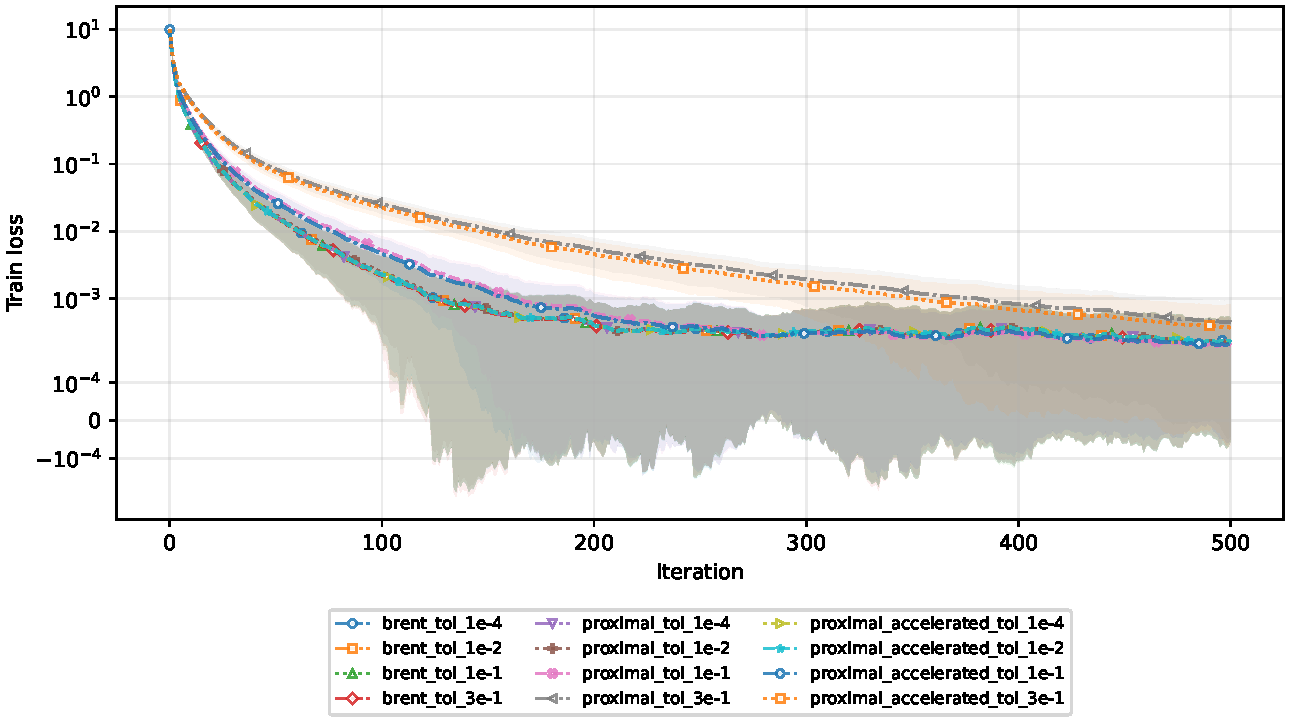
\includegraphics[width=\linewidth]{plots/quadratic_solver_comparison/train_loss_log.pdf}
    \caption{Training loss on a symmetric logarithmic scale. Lines show the
    mean and bands show one standard deviation on each side.}
    \label{fig:solver-train-loss}
\end{figure}

\begin{figure}[!htbp]
    \centering
    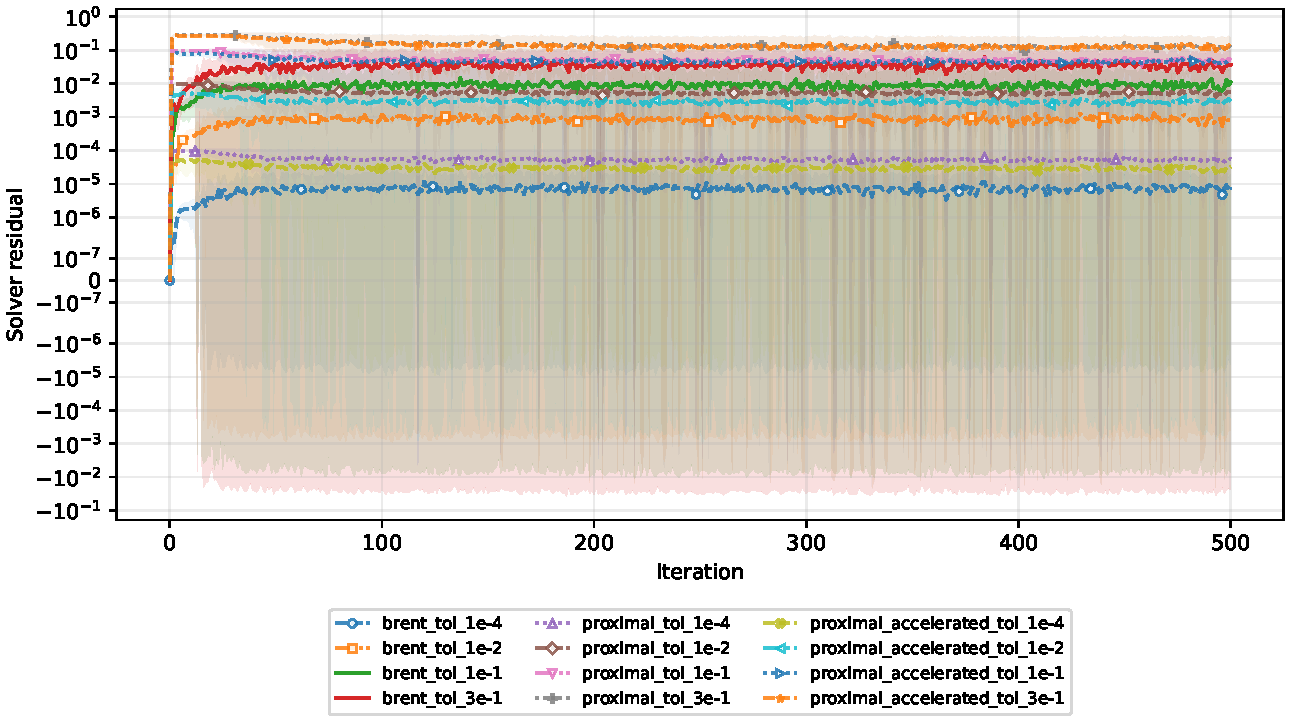
\includegraphics[width=\linewidth]{plots/quadratic_solver_comparison/solver_residual_log.pdf}
    \caption{Relative residual of the robust step at each outer iteration.
    Bands show the mean plus and minus one standard deviation.}
    \label{fig:solver-residual}
\end{figure}

\clearpage

\begin{figure}[!htbp]
    \centering
    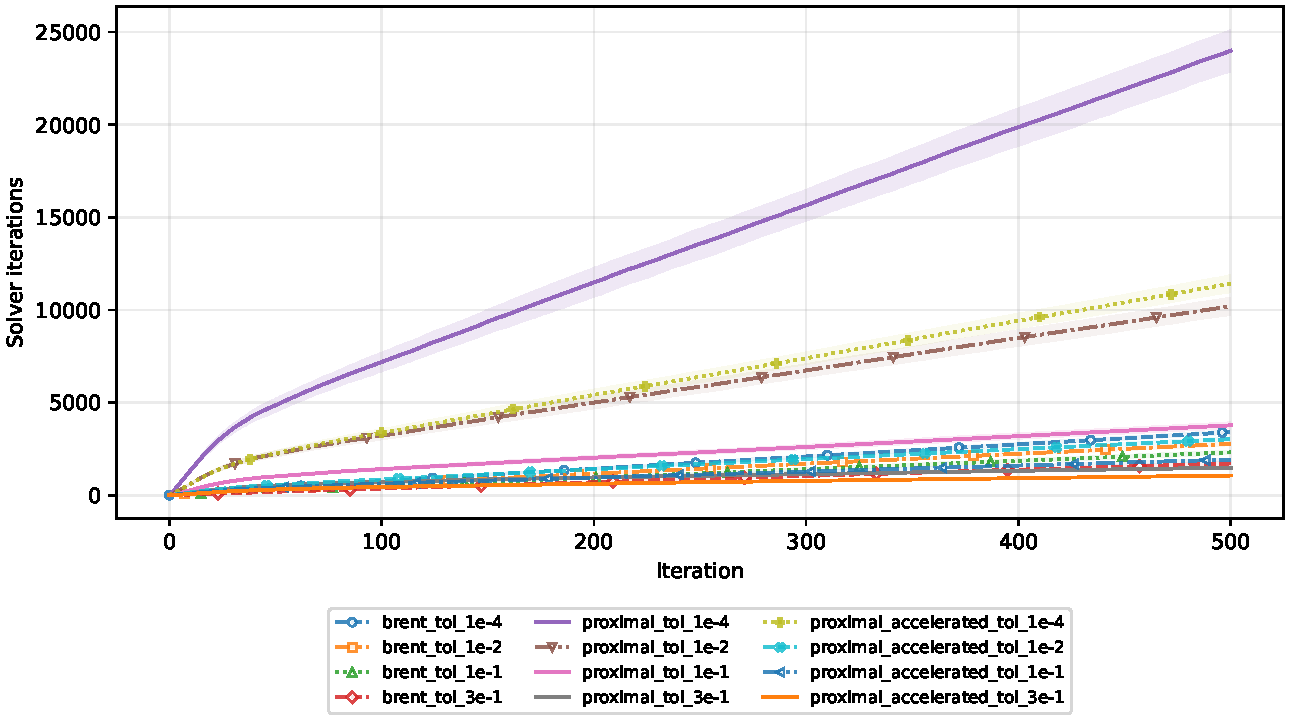
\includegraphics[width=\linewidth]{plots/quadratic_solver_comparison/solver_iterations.pdf}
    \caption{Cumulative inner work, shown as mean $\pm$ one standard
    deviation. The count is function evaluations for Brent and
    proximal updates for proximal gradient.}
    \label{fig:solver-work}
\end{figure}

\paragraph{Choice.}
We use Brent with tolerance $10^{-1}$ in the following experiments.
It matches the loss and stop step of Brent at $10^{-4}$ while using
about one third fewer function evaluations over 500 steps
(Figure~\ref{fig:solver-work}). Accelerated proximal at $10^{-2}$
gives similar loss with about 3025 proximal updates, compared with
2311 Brent evaluations. These counts describe different operations.
Brent at $3\cdot 10^{-1}$ uses fewer evaluations and reaches a similar
loss by step 500, but it triggers the outer stop rule about 35 steps
later on average. Tolerance $10^{-1}$ keeps the stop behavior close to
the tighter settings while reducing the inner work.

\begin{thebibliography}{9}
\bibitem{scipy-brent}
SciPy developers.
\href{https://docs.scipy.org/doc/scipy/reference/generated/scipy.optimize.minimize_scalar.html}
     {\texttt{scipy.optimize.minimize\_scalar}: documentation}.

\bibitem{parikh-boyd}
N.~Parikh and S.~Boyd.
\href{https://web.stanford.edu/~boyd/papers/pdf/prox_algs.pdf}
     {\emph{Proximal Algorithms}}.
\emph{Foundations and Trends in Optimization}, 1(3):123--231, 2014.
\end{thebibliography}

\end{document}
